\section{Membuat Fungsi Dalam Satu File dan Cara Menggunakannya}
Pada bagian ini terdapat tutorial cara membuat function yang berhubungan dengan “Akuisisi Data Menggunakan Sensor EEG”. Di bagian awal ini terdapat beberapa function yang disipan dalam satu file diantaranya adalah function untuk membuat tampilan, tampilan yang ada di tutorial ini terbagi ke dalam :
\begin{enumerate}
\item Membuat tampilan untuk mencari file.
\item Membuat tampilan untuk memilih file.
\item Membuat tampilan untuk mengubah ke line graph.
\item Membuat tampilan untuk mengubah ke bar graph.
\item Membuat tampilan “file tidak ada” jika file belum dipilih.
\end{enumerate}
Setelah itu ada function untuk :
\begin{enumerate} 
\item memilih file.
\item mengconvert file ke line graph.
\item Mengkonversi file ke bar graph.
\end{enumerate}
Pada bagian ini function akan dieksekusi oleh satu fungsi dalam file yang sama.
\subsection{Function untuk membuat tampilan awal}
Seperti pada listing \ref{lst:tampilanawal}:
\lstinputlisting[caption=Tampilan awal, label={lst:tampilanawal}]{src/3/tampilanawal.py}

Langkah pertama membuat tampilan
\begin{enumerate}
\item Membuat tampilan untuk mencari file.
Seperti pada listing \ref{lst:mencarifile}:
\lstinputlisting[caption=Tampilan untuk mencari file, label={lst:mencarifile}]{src/3/mencarifile.py}

\item Membuat tampilan untuk memilih file.
Seperti pada listing \ref{lst:memilihfile}:
\lstinputlisting[caption=Tampilan untuk memilih file, label={lst:memilihfile}]{src/3/memilihfile.py}

\item Membuat tampilan untuk mengubah ke line graph.
Seperti pada listing \ref{lst:linegraph}:
\lstinputlisting[caption=Tampilan line graph, label={lst:linegraph}]{src/3/linegraph.py}

\item Membuat tampilan untuk mengubah ke bar graph.
Seperti pada listing \ref{lst:bargraph}:
\lstinputlisting[caption=Tampilan bar graph, label={lst:bargraph}]{src/3/bargraph.py}

\item Kemudian function untuk memilih file.
Seperti pada listing \ref{lst:memilihfile2}:
\lstinputlisting[caption=Tampilan untuk memilih file, label={lst:memilihfile2}]{src/3/memilihfile2.py}
\begin{itemize}
\item Buat askopenfilename() yang bertujuan untuk memberikan pertanyaan file mana yang akan dipilih. 
\item Value nya dibuat float dengan menggunakan method split agar dapat mengembalikan lagi string line yang dipanggil.
\item Membuat function open agar bisa menampilkan menu open file.
\item Didefinisikan menjadi return jika file tidak ada dan bermaksud agar perintah tersebut bisa diulang-ulang.
\item Membuat x.append dan y.append untuk value di sumbu x dan sumbu y.
\item Membuat print file sudah tersedia dengan self dengan value “file sudah tersedia”.
\end{itemize}

\item Membuat function Line Graph.
Seperti pada listing \ref{lst:flinegraph}:
\lstinputlisting[caption=Tampilan function line graph, label={lst:flinegraph}]{src/3/flinegraph.py}
\begin{itemize}
\item Definisikan line\_graph menjadi self.
\item Membuat plt.figure dan variable num dengan value line graph dan file graph to converter untuk mengconvert data ke graph.
\item Buat plt.plot dengan value maker sebagai tanda sumbu x dan sumbu y.
\item Buat plt.xlabel sebagai title yang memberitahu panjang gelombang.
\item Buat plt.xlabel sebagai title yang memberitahu banyak gelombang.
\item Pada bagian ini data dibuat ke plt atau plot karena data akan disajikan ke dalam bentuk grafik.
\item Masing-masing plot didefinisikan sehingga tampilan grafik akan sesuai dan dapat dimengerti.
\item Buat plt.show untuk menampilkan hasil.
\end{itemize}

\item Kemudian mendefinisikan bar graph.
Seperti pada listing \ref{lst:fbargraph}:
\lstinputlisting[caption=Tampilan function bar graph, label={lst:fbargraph}]{src/3/fbargraph.py}
\begin{itemize}
\item Definisikan bar\_graph menjadi self.
\item Membuat plt.figure dan variable num dengan value line graph dan file graph to converter untuk mengconvert data ke graph.
\item Buat plt.plot dengan value maker sebagai tanda sumbu x dan sumbu y.
\item Buat plt.xlabel sebagai title yang memberitahu panjang gelombang.
\item Buat plt.xlabel sebagai title yang memberitahu banyak gelombang.
\item Pada bagian ini data dibuat ke plt atau plot karena data akan disajikan ke dalam bentuk grafik.
\item Masing-masing plot didefinisikan sehingga tampilan grafik akan sesuai dan dapat dimengerti.
\item Buat plt.show untuk menampilkan hasil.
\end{itemize}
\end{enumerate}

\section{Membuat Fungsi Pada File Terpisah Dari Cara Penggunaannya}
Pada bagian ini akan diberitahu bagaimana cara membuat function secara terpisah dalam file yang berbeda-beda tetapi dapat dijalankan oleh satu function. Function tersebut diantaranya:
\begin{enumerate}
\item Function membuka dan membaca file.
\item Function Untuk Menjalankan.
\item Function Menampilkan Data
\item Function Untuk Menampilkan Gelombang.
\item Function Menampilkan Gelombang Dengan Marker.
\item Function Membuat Titile Pada Grafik.
\item Function Membuat Keterangan Pada Sumbu X.
\item Function Membuat Keterangan Pada Sumbu Y.
\item Membuat fungsi untuk menampilkan row di sumbu x dan sumbu y.
\item Function Membuat warna pada row.
\item Membuat scatter
\end{enumerate}

Pada bagian dua, fungsi dibuat secara terpisah pada file yang berbeda-beda dan hanya dapat menjalankan fungsi itu saja tidak bisa berbarengan dengan fungsi yang lain. Dan perintah untuk menjalankannya ada di dalam fungsi tersebut.
\begin{enumerate}
\item Function membuka dan membaca file.
Seperti pada listing \ref{lst:membacafile}:
\lstinputlisting[caption=Tampilan function membuka dan membaca file, label={lst:membacafile}]{src/3/membacafile.py}
\begin{itemize}
\item Buat f sebagai objek/variable yang menampung isi file. 
\item Kemudian pilih file yang akan diambil sebagai data.
\item Buat print dan f.read agar data kemudian dibaca dan dicetak.
\end{itemize}

\item Function Untuk Menjalankan.
Seperti pada listing \ref{lst:main}:
\lstinputlisting[caption=main.py, label={lst:main}]{src/3/main.py}
\begin{itemize}
\item Pada bagian ini awalnya kita mengimport mindwave, maksudnya adalah agar dapat mengambil data di alat pembaca sinyal. 
\item Setelah itu membuat variable headset yang berisikan data yang ada di computer, headset tadi kita isi dengan COM4 sesuai dengan computer yang anda gunakan.

Seperti pada listing \ref{lst:com}:
\lstinputlisting[caption=Pilih COM, label={lst:com}]{src/3/com.py}

\item Setelah itu membuat fungsi koneksi atau menghubungkan
Seperti pada listing \ref{lst:koneksi}:
\lstinputlisting[caption=Koneksi, label={lst:koneksi}]{src/3/koneksi.py}

\item Kita definisikanJika data di mindwave belum terhubung maka laptop akan mencoba menghubungkan kembali, jika sudah ada maka akan muncul “connected”.
\end{itemize}

\item Function Menampilkan Data
Seperti pada listing \ref{lst:tampildata}:
\lstinputlisting[caption=Function Menampilkan Data, label={lst:tampildata}]{src/3/tampildata.py}
\begin{itemize}
\item Membuat img = img.open sebagai function untuk memilih gambar, kemudian dipilih gambar yang akan ditampilkan.
\item Membuat variable draw.
\item Data diambil dan dimasukan.
\item Data yang ada akan diimport ke dalam bentuk gambar dan ditampilkan.
\end{itemize}

\item Function Untuk Menampilkan Gelombang.
Seperti pada listing \ref{lst:tampilgelombang}:
\lstinputlisting[caption=Function Menampilkan Gelombang, label={lst:tampilgelombang}]{src/3/tampilgelombang.py}
\begin{itemize}
\item Pertama-tama import dulu data matplotlib menjadi plot agar mudah mendefinisikan data menjadi sebuah plot. 
\item Setelah itu buatlah variable plot agar dapat membaca file csv.
\item Csv.reader agar python dapat membaca format csv.
\item Kemudian buat plt.show agar data gelombang dalam bentuk grafik dapat ditampilkan.
\end{itemize}

\item Function Menampilkan Gelombang Dengan Marker.
Seperti pada listing \ref{lst:maker}:
\lstinputlisting[caption=Function Menampilkan Gelombang Dengan Maker, label={lst:maker}]{src/3/maker.py}
\begin{itemize}
\item Pertama-tama import dulu data matplotlib menjadi plot agar mudah mendefinisikan data menjadi sebuah plot.
\item Setelah itu buatlah variable plot agar dapat membaca file csv.
\item Kemudian buat fungsi plot dan isi valuenya dengan (x, marker=’o’) untuk membuat sumbu x dan o.
\item Kemudian buat plt.show agar data gelombang dalam bentuk grafik dapat ditampilkan.
\end{itemize}

\item Function Membuat Title Pada Grafik.
Seperti pada listing \ref{lst:title}:
\lstinputlisting[caption=Function Membuat Title Pada Grafik, label={lst:title}]{src/3/title.py}
\begin{itemize}
\item Pertama-tama import dulu data matplotlib menjadi plot agar mudah mendefinisikan data menjadi sebuah plot. 
\item Setelah itu buatlah variable plot agar dapat membaca file csv.
\item Kemudian buat fungsi plot da nisi valuenya dengan (x, marker=’o’) untuk membuat sumbu x dan o.
\item Kemudian buat fungsi plt.title da nisi valuenya sesuai yang diinginkan.
\end{itemize}

\item Function Membuat Keterangan Pada Sumbu X.
Seperti pada listing \ref{lst:xlabel}:
\lstinputlisting[caption=xlabel, label={lst:xlabel}]{src/3/xlabel.py}
\begin{itemize}
\item Pertama-tama import dulu data matplotlib menjadi plot agar mudah mendefinisikan data menjadi sebuah plot. 
\item Setelah itu buatlah variable plot agar dapat membaca file csv.
\item Kemudian buat fungsi plot da nisi valuenya dengan (x, marker=’o’) untuk membuat sumbu x dan o.
\item Kemudian buat fungsi plt.title da nisi valuenya sesuai yang diinginkan.
\item Buat plt.xlabel untuk keterangan di sumbu x.
\end{itemize}

\item Function Pembuatan Rows dan Scatter 
Seperti pada listing \ref{lst:warnascatter}:
\lstinputlisting[caption=Warna Scatter, label={lst:warnascatter}]{src/3/warnascatter.py}
\begin{itemize}
\item Pertama-tama import dulu data matplotlib menjadi plot agar mudah mendefinisikan data menjadi sebuah plot. 
\item Setelah itu buatlah variable plot agar dapat membaca file csv.
\item Kemudian buat fungsi plot da nisi valuenya dengan (x, marker=’o’) untuk membuat sumbu x dan o.
\item Setelah itu buat fungsi plt.title untuk judul di atas.
\item Buat plt.xlabel untuk keterangan di sumbu x.
\item Buat plt.ylabel untuk keterangan di sumbu y.
\item Setelah itu buat fungsi x.append untuk sumbu x.
\item Buat fungsi y.append untuk sumbu y agar di setiap sumbu terdapat row tingkatan jumlah data.
\item Buat plt.hist dengan value facecolor dan definisikan warnanya.
\item Setelah itu membuat fungsi scatter untuk sumbu x.
\item Setelah itu membuat fungsi scatter untuk sumbu y agar gelombang dan row dapat dibaca dengan pas.
\item Tambahkan scatter facecolor pada x dan y.
\end{itemize}
\end{enumerate}

\section{Membuat Kelas dan Cara Instalasi Kelas Pada Program Utama}
Pada bagian ini akan dibahas cara membuat kelas dan cara memanggil kelas tersebut pada program utama. Pertama-tama buatlah kelas terlebih dahulu.

Seperti pada listing \ref{lst:class}:
\lstinputlisting[caption=Membuat Kelas, label={lst:class}]{src/3/class.py}
	
Langkah selanjutnya buatlah dua objek yang sama-sama memanggil class tersebut.
Seperti pada listing \ref{lst:object}:
\lstinputlisting[caption=Membuat Objek Kelas, label={lst:object}]{src/3/object.py}

\section{Hasil Pengujian}
\subsection{Tampilan awal}
Hasilnya seperti pada gambar \ref{fig:tampilanawal}:
\begin{figure}[!htbp]
	\centerline{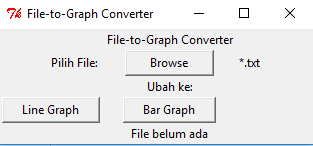
\includegraphics[width=0.85\textwidth]{figures/3/tampilanawal.PNG}}
	\caption{Tampilan awal}
	\label{fig:tampilanawal}
\end{figure}

\subsection{Tampilan Pilih File}
Hasilnya seperti pada gambar \ref{fig:tampilanpilih}:
\begin{figure}[!htbp]
	\centerline{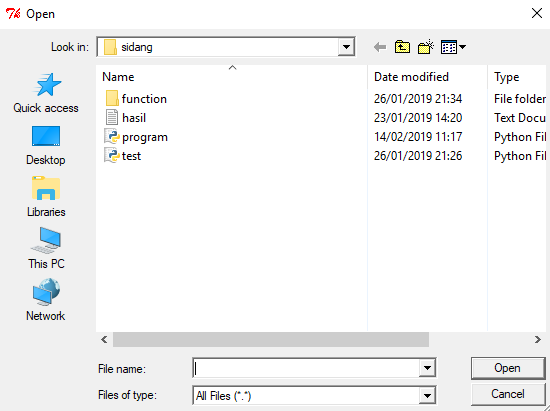
\includegraphics[width=0.85\textwidth]{figures/3/tampilanpilih.PNG}}
	\caption{Tampilan pilih file}
	\label{fig:tampilanpilih}
\end{figure}

\subsection{Tampilan line graph}
Hasilnya seperti pada gambar \ref{fig:linegraph}:
\begin{figure}[!htbp]
	\centerline{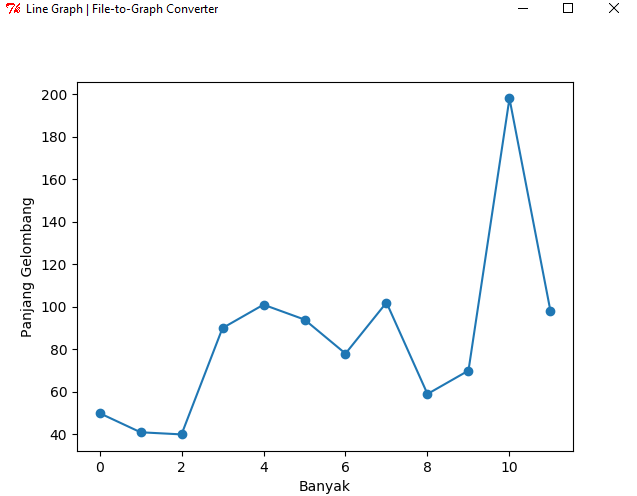
\includegraphics[width=0.85\textwidth]{figures/3/linegraph.PNG}}
	\caption{Data line graph}
	\label{fig:linegraph}
\end{figure}

\subsection{Tampilan Bar Graph}
Hasilnya seperti pada gambar \ref{fig:bargraph}:
\begin{figure}[!htbp]
	\centerline{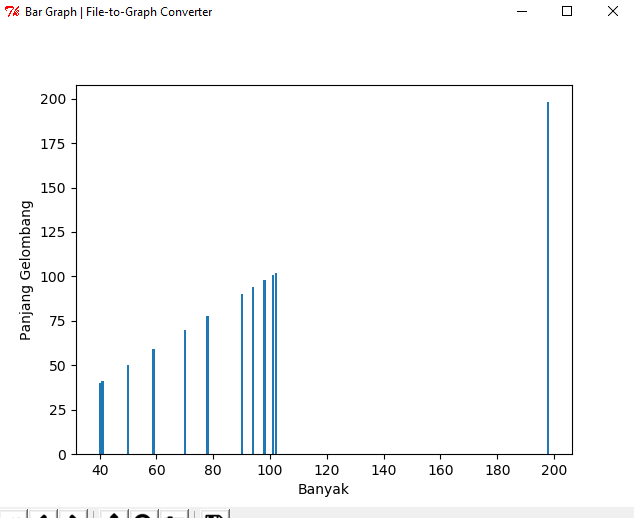
\includegraphics[width=0.85\textwidth]{figures/3/bargraph.PNG}}
	\caption{Data bar graph}
	\label{fig:bargraph}
\end{figure}

\section{PENANGANAN ERROR PADA PYTHON}
\subsection{Penanganan error}
Saat menjalankan program terkadang program tidak jalan/tidak dapat dieksekusi, untuk menangani hal tersebut harus diketahui terlebih dahulu errornya, setelah error diketahui maka program dapat dijalankan kembali. Error yang terjadi pada saat menjalankan program di python terbagi menjadi dua yaitu error pada penulisan syntax dan error pada logika yang diperintahkan dalam program. Karena suatu python tidak akan mengerti perintah yang dimasukkan jika program tersebut terdapat kesalahan dan tidak dapat dimengerti oleh computer.

\begin{enumerate}
\item Kesalahan syntax

Kesalahan syntax biasanya terjadi dalam kesalahan penulisan, jika syntax tidak ada dalam python dan tidak bisa dipahami maka python akan menunjukkan adanya kesalahan dalam program tersebut. Untuk mengatasi error dalam penulisan syntax maka pembuat program harus lebih teliti lagi dalam pengetikan saat memberikan perintah di python.

Berikut adalah contoh error yang terjadi karena kesalahan syntax seperti pada gambar \ref{fig:salahsintak}
\begin{figure}[!htbp]
	\centerline{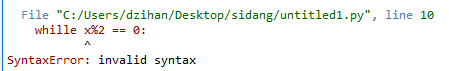
\includegraphics[width=0.85\textwidth]{figures/3/salahsintak.PNG}}
	\caption{Kesalahan sintak}
	\label{fig:salahsintak}
\end{figure}
	
Gambar \ref{fig:salahsintak} adalah contoh error yang terjadi yang disebabkan oleh kesalahan dalam penulisan syntax. Hal tersebut terjadi karena dalam program tersebut terdapat ‘kata’ atau perintah yang tidak dapat dipahami oleh komputer.

Untuk menangani hal tersebut maka periksa lagi lagi atau klik errornya seperti pada listing \ref{lst:syntaxsolution}:
\lstinputlisting[caption=Solusi Kesalahan Sintak, label={lst:syntaxsolution}]{src/3/syntaxsolution.py}

\item Kesalahan logika
Selain kesalahan syntax ada juga kesalahan logika. Kesalahan logika terjadi akibat terdapat logika yang tidak dapat dipahami dalam program yang dibuat seperti pada gambar \ref{fig:salahlogika}
\begin{figure}[!htbp]
	\centerline{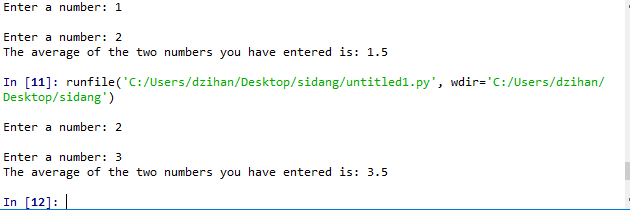
\includegraphics[width=0.85\textwidth]{figures/3/salahlogika.PNG}}
	\caption{Kesalahan logika}
	\label{fig:salahlogika}
\end{figure}

Untuk memperbaiki error tersebut cukup dengan menambahkan tanda kurung dalam rumusnya seperti pada listing \ref{lst:logicsolution}:
\lstinputlisting[caption=Solusi Kesalahan Logika, label={lst:logicsolution}]{src/3/logicsolution.py}:
\end{enumerate}

\subsection{Fungsi memilih line graph}
Seperti pada listing \ref{lst:linegraph2}:
\lstinputlisting[caption=Line Graph, label={lst:linegraph2}]{src/3/linegraph2.py}

Seperti pada gambar \ref{fig:errorplt}
\begin{figure}[!htbp]
	\centerline{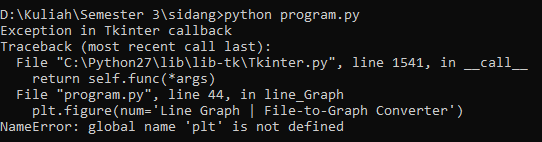
\includegraphics[width=0.85\textwidth]{figures/3/errorplt.PNG}}
	\caption{Error plt}
	\label{fig:errorplt}
\end{figure}

Pada bagian awal terdapat exeption pada bagian tkinter, karena untuk menjalankan fungsi plot diperlukan adanya sebuah import terlebih dahulu dari matplotlib agar data dapat dibaca dan dikonversi ke plot.

Pada bagian ini terdapat error yang menunjukan bahwa global name dengan nama plt tidak terdefinisikan. Dalam fungsi pengambilan data, data diharuskan diimport dulu ke plot dengan menggunakan matplotlib agar data dapat disajikan dalam bentuk plot. Agar lebih mudah didefinisikan, maka matplotlib menggunakan “as” atau alias sebagai plt. 

Untuk menangani error tersebut ada beberapa langkah yang harus dikerjakan :
\begin{enumerate}
\item Import matplotlib.pyplot
\item buat lah “as” atau alias pada bagian import matplotlib agar fungsi yang ada di line\_graph dapat mendefinisikan plt tersebut sebagai matplotlib.
\item Pada bagian fungsi line\_graph harus didefinsikan sama seperti alias yang telah ditentukan
Seperti pada listing \ref{lst:import}:
\lstinputlisting[caption=Import, label={lst:import}]{src/3/import.py}
\item Setelah dibuat langkah-langkah tersebut maka function dapat dijalankan kembali dan function line graph dapat mendefinisikan plt sebagai matplotlib.
\end{enumerate}

\subsection{Fungsi memilih file}
Seperti pada listing \ref{lst:choosefile}:
\lstinputlisting[caption=Memilih file, label={lst:choosefile}]{src/3/choosefile.py}

\begin{figure}[!htbp]
	\centerline{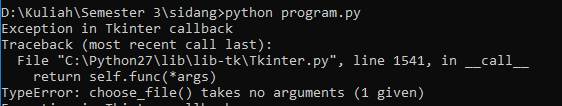
\includegraphics[width=0.85\textwidth]{figures/3/errorcf.PNG}}
	\caption{Error Choose File}
	\label{fig:errorcf}
\end{figure}
Pada gambar \ref{fig:errorcf} terdapat error exception bagian type error, yang menunjukan bahwa ada error di bagian choose file dan adanya sebuah fungsi yang dieksekusi dengan type objek yang tidak sesuai.

Untuk menangani hal tersebut perlu dibuat parameter self, jika sebuah method yang ada pada dirinya sendiri harus diawali dengan self.
Seperti pada listing \ref{lst:selfcf}:
\lstinputlisting[caption=Self Choose File, label={lst:selfcf}]{src/3/selfcf.py}

self.adaFile["text"]="File sudah tersedia!" Pada bagian ini sebelum menjalankan perintah “adaFile” dan memunculkan print “file sudah tersedia, self akan memanggil dirinya sendiri terlebih dahulu kemudia menjalankan perintah “adaFile”. Itulah kegunaan self dan hasil dari penanganan error menggunakan self membuat fungsi choose file dapat dijalankan kembali.

Seperti pada gambar \ref{fig:selfcf}
\begin{figure}[!htbp]
	\centerline{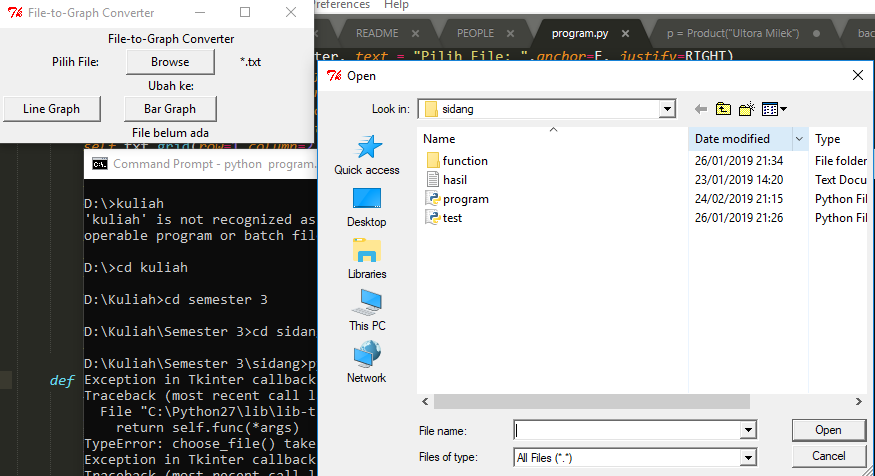
\includegraphics[width=0.85\textwidth]{figures/3/selfcf.PNG}}
	\caption{Self Choose File}
	\label{fig:selfcf}
\end{figure}

Seperti pada listing \ref{lst:file_name}:
\lstinputlisting[caption=file\_name, label={lst:file_name}]{src/3/file_name.py}

\begin{figure}[!htbp]
	\centerline{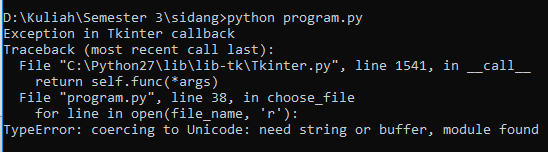
\includegraphics[width=0.85\textwidth]{figures/3/file_name.PNG}}
	\caption{Error file\_name}
	\label{fig:file_name}
\end{figure}
Pada gambar \ref{fig:file_name} memberitahu exeption yang terjadi pada fungsi memilih file, tepatnya pada bagian file\_name. Exeption yang tertera di gambar adalah TypeError yang memberitahu bahwa method tersebut membutuhkan string.

Seperti pada listing \ref{lst:openfile}:
\lstinputlisting[caption=open\_file, label={lst:openfile}]{src/3/openfile.py}
	
Pada bagian ini terdapat perintah open yang memanggil file\_name dan r, namun r disini tidak dapat ditemukan. Maka penaganan error untuk bagian ini adalah sebagai berikut :
\begin{enumerate}	
\item Definisikan r menjadi askopenfile agar r dapat menjalankan sebuah perintah. file\_name = filedialog.askopenfilename().
\end{enumerate}

\section{Tutorial Penanganan Error Pada Tkinter}
Pada pembuatan sebuah tampilan menggunakan GUI, maka harus menggunakan tkinter untuk dapat menampilkan interface berbentuk menu GUI. Dalam penggunaan tkinter sering terdapat kesalahan/error saat proses import tkinter ke python. Seperti pada gambar \ref{fig:errortkinter}
\begin{figure}[!htbp]
	\centerline{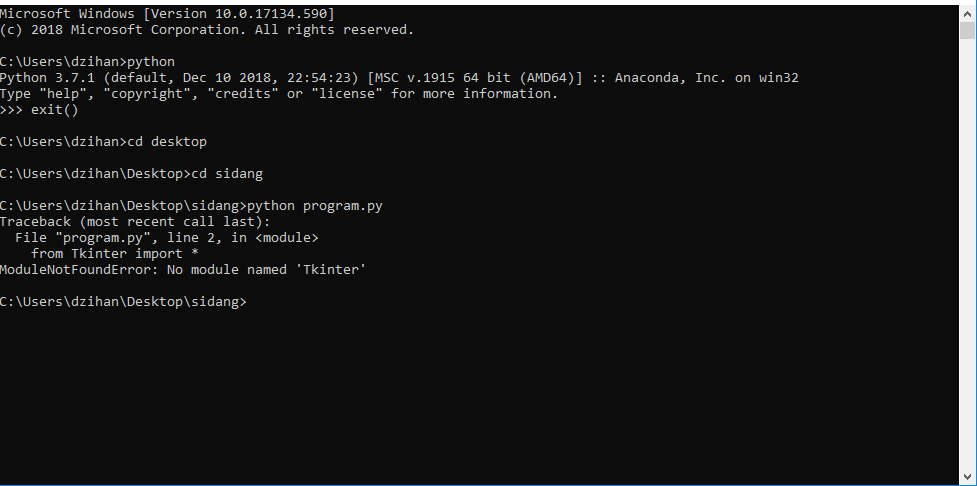
\includegraphics[width=0.85\textwidth]{figures/3/errortkinter.PNG}}
	\caption{Error Tkinter}
	\label{fig:errortkinter}
\end{figure}

Dalam kasus error tersebut python tidak dapat menampilkan program.py karena tidak terdapat modul tkinter. Dalam program.py tersebut ada source code yang diperintahkan untuk menampilkan menu GUI, dalam menu GUI tersebut terdpat fungsi-fungsi. JIka menu tidak bisa diakses maka fungsi pun tidak akan dapat dijalankan. Untuk menangani error tersebut perlu dilakukan import tkinter.
\begin{enumerate}
\item Buka cmd
\item Buka python
\item Ketik Import tkinter

Seperti pada listing \ref{lst:tkinter}:
\lstinputlisting[caption=Import Tkinter, label={lst:tkinter}]{src/3/tkinter.py}

Seperti pada gambar \ref{fig:tkinter}
\begin{figure}[!htbp]
	\centerline{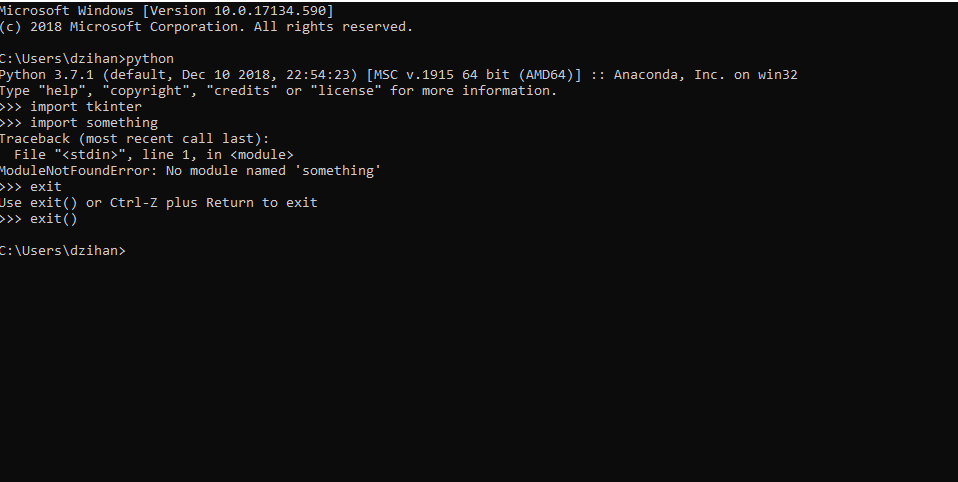
\includegraphics[width=0.85\textwidth]{figures/3/tkinter.PNG}}
	\caption{Import Tkinter}
	\label{fig:tkinter}
\end{figure}

\item Kemudian buka instalasi python yang telah didownload.
Seperti pada gambar \ref{fig:folderpython}
\begin{figure}[!htbp]
	\centerline{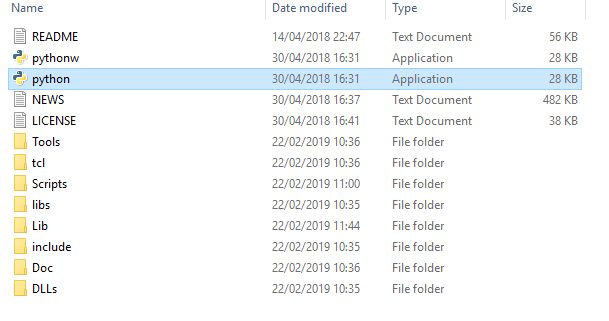
\includegraphics[width=0.85\textwidth]{figures/3/folderpython.PNG}}
	\caption{Folder Python}
	\label{fig:folderpython}
\end{figure}

\item Arahkan atau drop ke cmd
Seperti pada gambar \ref{fig:dropfolder}
\begin{figure}[!htbp]
	\centerline{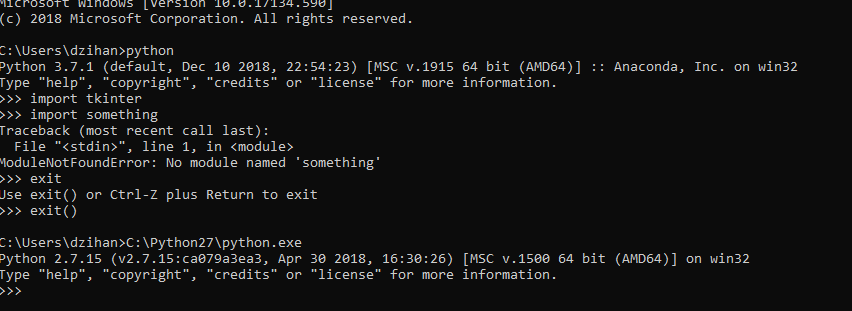
\includegraphics[width=0.85\textwidth]{figures/3/dropfolder.PNG}}
	\caption{Drop Folder}
	\label{fig:dropfolder}
\end{figure}

\item Setelah itu import kembali tkinter
\end{enumerate}

Jika cara tersebut tidak berhasil, cobalah cara lain seperti tutorial di bawah ini :
\begin{enumerate}
\item Buka folder python.
Seperti pada gambar \ref{fig:bukafolder}
\begin{figure}[!htbp]
	\centerline{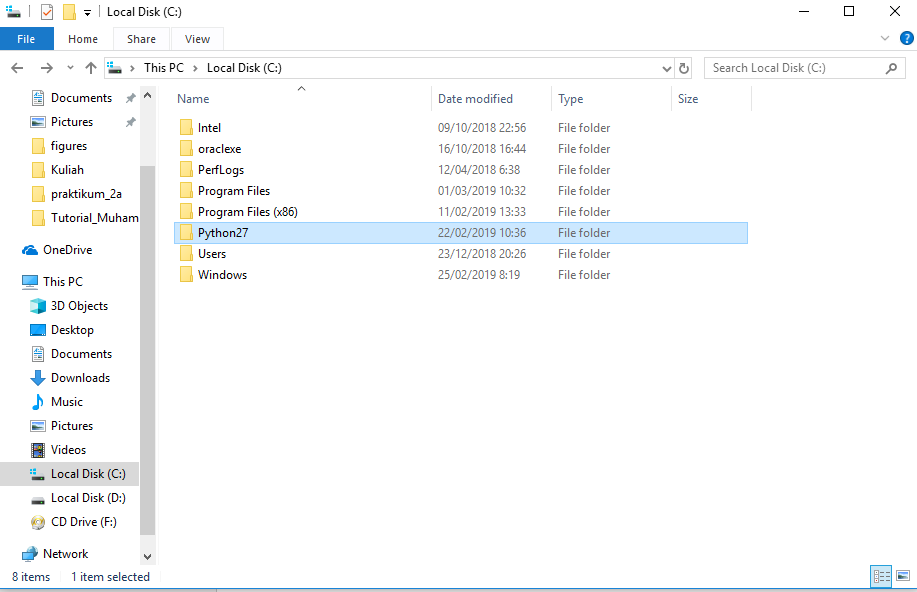
\includegraphics[width=0.85\textwidth]{figures/3/bukafolder.PNG}}
	\caption{Buka Folder Python}
	\label{fig:bukafolder}
\end{figure}

\item Buka cmd
\item Tambahkan folder python tadi ke cmd.
Seperti pada gambar \ref{fig:tambahfolder}
\begin{figure}[!htbp]
	\centerline{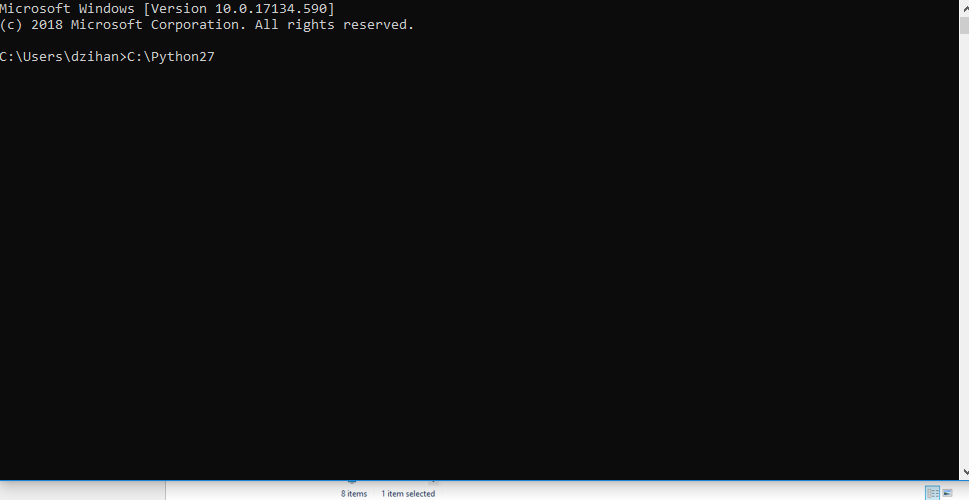
\includegraphics[width=0.85\textwidth]{figures/3/tambahfolder.PNG}}
	\caption{Tambahkan Folder}
	\label{fig:tambahfolder}
\end{figure}

\item Ketik pip install “nama modul”
Seperti pada listing \ref{lst:pipinstall}:
\lstinputlisting[caption=Pip install "nama modul", label={lst:pipinstall}]{src/3/pipinstall.py}

Seperti pada gambar \ref{fig:installmodul}
\begin{figure}[!htbp]
	\centerline{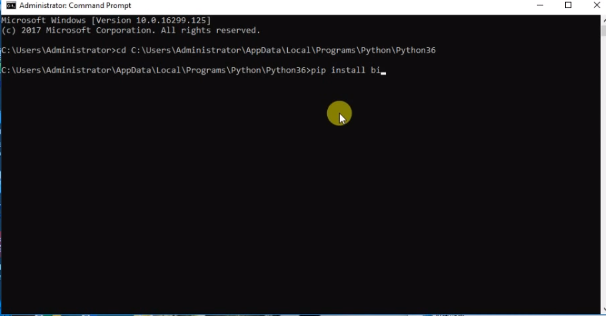
\includegraphics[width=0.85\textwidth]{figures/3/installmodul.PNG}}
	\caption{Install Modul}
	\label{fig:installmodul}
\end{figure}

\item Modul sudah tersedia
Seperti pada gambar \ref{fig:atkinter}
\begin{figure}[!htbp]
	\centerline{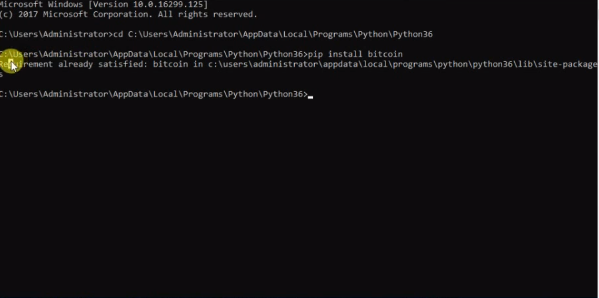
\includegraphics[width=0.85\textwidth]{figures/3/atkinter.PNG}}
	\caption{Modul sudah tersedia}
	\label{fig:atkinter}
\end{figure}
\end{enumerate}